% LAB Final: Phonebook Project
%
% CSE/IT 107: Introduction to Programming
% New Mexico Tech
%
\documentclass[11pt]{cselabheader}

%%%%%%%%%%%%%%%%%% SET TITLES %%%%%%%%%%%%%%%%%%%%%%%%%
\fancyhead[R]{Final Project: Phone Book}
\title{Final Project: Phone Book}

\begin{document}

\maketitle
\pagenumbering{roman}
\hrule

\begin{figure}[H]
\centering
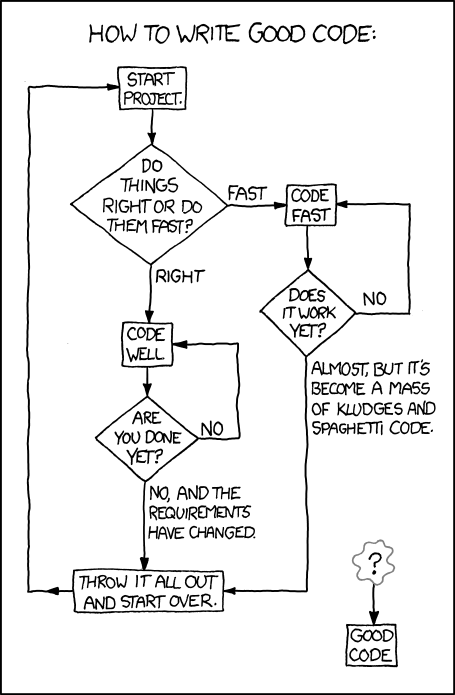
\includegraphics[width=0.5\textwidth]{img/xkcd_good_code.png}
\caption{XKCD on how to write good code \url{https://xkcd.com/844/}.}
\end{figure}

\hrule

\pagebreak
\tableofcontents

\begin{figure}[H]
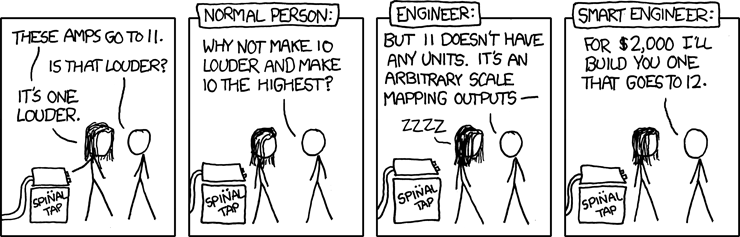
\includegraphics[width=\textwidth]{img/xkcd_spinal_tap_amps.png}
\caption{XKCD on engineers \url{https://xkcd.com/670/}.}
\end{figure}

\pagebreak
\pagenumbering{arabic}

\section{The Problem}

You are an employee of NMTLabs a small software consultation firm for
noble gas mass spectrometry. At this week's weekly developer's meeting
you were tasked with developing an application to manage the firm's
contacts. The CEO and CTO of NMTLabs are looking for something that is
text-based and easy to use, so the firm can quickly start calling
contacts for the latest round of venture capital fundraising.
Heretofore the firm has been using a simple CSV file to save all of
its contacts.  Everyone in the organization is looking for an improved
solution and are counting on you to have a working prototype.

The CTO has specified a set of tasks your contacts application must
perform. Please examine the requirements carefully, implement as many
of the tasks as possible including the Extra Credit (E.C worth 1\%
each)

\subsection{Example Session}
An example session using the application is show below. A user starts
the application, enters the commands, about, info, list and finally
exit.  The application displays a farewell message and quits.

%%% fill in
\begin{verbatimcode}
\end{verbatimcode}

\section{Assignment}
Make your code clean and readable. You will be graded on style and
functionality.  \textbf{You must follow PEP8 and PEP257}.

\subsection{Documentation}
Write a \texttt{README.txt} file. This is common practice in the open
source community and provides a consistent location for users to find
introductory information about your application. This file should
contain a brief description of what your code does and some
information on how to run it.  You should provide a list of valid
commands, their function, and examples of their use.

\subsection{Contacts Format}
A contact is something that stores least the following attributes:
\begin{itemize}
\item Name
\item Phone
\item Company
\item Email
\item Note %%% remove?
\end{itemize}

Here is a sample CSV file describing many contacts.

\begin{verbatimcode}
Name, Phone, Company, Email, Note
%%% make something up
\end{verbatimcode}

\subsection{Application}
%%% application modes; how to switch

%%% suggestion: to make testing easier, hardcode some contacts

\subsubsection{The \texttt{exit} and \texttt{about} Commands}

\subsubsection{The \texttt{info} Command}

\subsubsection{The \texttt{list} and \texttt{lookup} Commands}

\subsubsection{The \texttt{remove} Command}

\subsubsection{The \texttt{add} Command}

\subsubsection{The \texttt{load} Command}

\subsubsection{The \texttt{save} Command}
%%% writing a CSV file should be easy:
%%% include this anyway?
%%% \pythoninline{savefile.write("{}, {}, {}, {}, {}\n", name, phone, company, email, note)}

\subsection{Extra Credit}

\newpage
\section{Submitting}

You should submit your code as a tarball. It should contain all files
used in solving the problems presented in this lab. The submitted file
should be named
\begin{center}
  \texttt{cse107\_firstname\_lastname\_.tar.gz}
\end{center}

\begin{center}
  \textbf{Upload your tarball to Canvas.}
\end{center}

\end{document}


